\documentclass[11pt, oneside]{article}   	% use "amsart" instead of "article" for AMSLaTeX format
\usepackage{geometry}                		% See geometry.pdf to learn the layout options. There are lots.
\geometry{letterpaper}                   		% ... or a4paper or a5paper or ... 
%\geometry{landscape}                		% Activate for for rotated page geometry
%\usepackage[parfill]{parskip}    		% Activate to begin paragraphs with an empty line rather than an indent
\usepackage{graphicx}				% Use pdf, png, jpg, or eps� with pdflatex; use eps in DVI mode
								% TeX will automatically convert eps --> pdf in pdflatex		
\usepackage{amssymb}
\usepackage{amsmath}
\usepackage{parskip}
\usepackage{color}

\title{Green's Theorems (work and flux)}
%\author{The Author}
%\section{}
% \subsection*{R code}
\date{}							% Activate to display a given date or no date

\graphicspath{{/Users/telliott_admin/Dropbox/Tex/png/}}

% \begin{center} 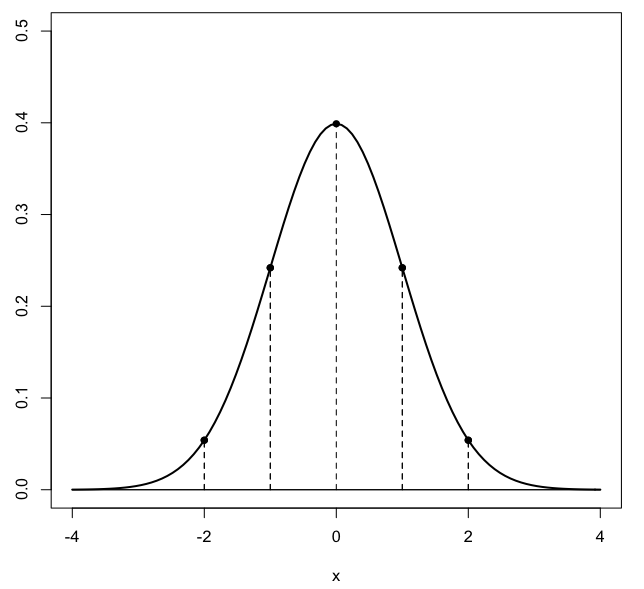
\includegraphics [scale=0.4] {gauss3.png} \end{center}
% \begin{bmatrix} a  &  b \\ c  &  d \end{bmatrix}
% \bigg |_

\begin{document}
\maketitle
\large
%\noindent
This short write-up will summarize the first two of the four fundamental theorems of vector calculus.  I hope this will help me to remember them.

First, though, a word about curl.  Curl measures the rotation of a vector field (its absolute value is twice the angular momentum).  As an example, if a two dimensional field $\mathbf{F}$ has components $<M,N>$, then
\[ \text{curl} \ \mathbf{F} = N_x - M_y \]

As we'll see, the calculation of $\text{curl} \ \mathbf{F}$ produces a vector, in this case it points out of the plane.  When we calculate with it in 2D we are implicitly dotting it with $\hat{\mathbf{k}}$.

Our convention is that we go on a curve around a region with $R$ on our left, then the curl points up.  

If the value of $\text{curl} \ \mathbf{F}$ is zero, then the work done going around the closed curve is also zero, alternatively if the curl is non-zero, work is done.  Think of swimming in a whirlpool.  Against the flow it is hard going, whereas with the flow, it's easy.

In our theorems, the curl will always be associated with the line integral for work.

The work done in moving along a curve $C$ is

\[ W = \int_C \mathbf{F} \cdot d\mathbf{r}  \]
\[ = \int_C \mathbf{F} \cdot \hat{\mathbf{T}} \ ds \]

In three dimensions, we use the "del" operator
\[ \nabla = \ < \frac{\partial}{\partial x},\frac{\partial}{\partial y},\frac{\partial}{\partial z} > \]

The curl of $\mathbf{F}$ is
\[ \nabla \times \mathbf{F} \]
For $\mathbf{F} = \ <P,Q,R>$
\[ \nabla \times \mathbf{F} =  \ <R_y-Q_z,P_z-R_x,Q_x-P_y> \]
which is basically impossible to remember except by using this convenient device
\[
\begin{vmatrix} 
  \hat{i}  &  \hat{j} & \hat{k} \\ 
  \frac{\partial}{\partial x}  &  \frac{\partial}{\partial y} & \frac{\partial}{\partial z} \\ 
  P  &  Q & R \\ 
\end{vmatrix} \ \ 
\]
In two dimensions $R=0$ and also $P_z$ and $Q_z$ are both zero, so this equation reduces to the one we saw above (substituting $M$ for $P$ and $N$ for $Q$).

A basic fact in vector calculus is that if the field is the gradient of a potential function, the curl is zero.  Let the function be $f$ and the field $\mathbf{F} = \nabla f$, then $M=f_x$ and $N=f_y$.  Then the curl is $f_{yx}- f_{xy}$, but for any such function
\[ f_{xy} = f_{yx} \]

\subsection*{Calculating}
Let's look again at
\[ W = \int_C \mathbf{F} \cdot d\mathbf{r} \]
\[  = \int_C \mathbf{F} \cdot \hat{\mathbf{T}} \ ds \]
This can be written as
\[ = \int_C M \ dx + N \ dy  \]
One way to see this is to say
\[ d\mathbf{r} = \frac{d}{dt} \mathbf{r} \ dt = \ <\frac{dx}{dt},\frac{dy}{dt}> \ dt \]
so when we do the dot product with $\mathbf{F}$, we get what we wrote above.

There is another important integral to be explained below
\[ \int_C \mathbf{F} \cdot \hat{\mathbf{n}} \  ds = \int_C -N \ dx + M \ dy  \]

It's really important to appreciate that although these equations look something like a double integral, they are \emph{not}.  We will have a parametrization of the curve in terms of $t$ (or $x$ or $\theta$), and a single integral like $\int_C \ [ \ \ ] \ dt $.

\subsection*{Green---work}
We start with two theorems in the plane (typically the $xy$-plane).  These are called Green's Theorem for work, and Green's Theorem for flux.  

Green's Theorem for work states that for a closed path

\[ \oint \mathbf{F} \cdot d\mathbf{r}  = \iint_R \ \nabla \times \mathbf{F} \ dA \]

One sticky point I had here is that the curl produces a vector, yet the formula is usually given as above.  That's because this is a special case of Stokes theorem where the term on the right is really 
\[ (\nabla \times \mathbf{F}) \cdot \hat{\mathbf{k}} \ dA \]
which (since $\nabla \times \mathbf{F} $ is parallel to $\hat{\mathbf{k}}$) gives what we have above.

Alternatively 

\[ \int_C M \ dx + N \ dy = \iint_R (N_x - M_y) \ dx \ dy \]

The work done along a closed path around $R$ is equal to the double integral over $R$ of the curl of $\mathbf{F}$.  Remember the whirlpool.

\subsection*{Green---flux}
Flux is flow across a curve, or in $R3$, through a surface.

Green's Theorem for flux (in the plane) states that for a closed path $C$ over a region $R$

\[ \int_C \mathbf{F} \cdot \hat{\mathbf{n}} \  ds = \iint_R \ \nabla \cdot \mathbf{F} \ dA \]
Alternatively
\[ \int_C M dy - N dx =  \iint_R \ (M_x + N_y) \ dx \ dy \]

Another use of the "del" operator is the divergence of $\mathbf{F}$

\[ \nabla \cdot \mathbf{F} \]
if $\mathbf{F} = \ <M,N>$
\[ \nabla \cdot \mathbf{F} = M_x + N_y \]

The divergence of a vector field is a scalar quantity.  It measures the net production (or disappearance) of the "substance" that flows in a vector field.  If there are no sources or sinks in a region, the divergence of $\mathbf{F}$ will be zero.

Restating the theorem:

\[ \oint \mathbf{F} \cdot \hat{\mathbf{n}} \ dS  = \iint_R \ \nabla \cdot \mathbf{F} \ dA \]

Breaking this down, on the left hand side of the first version, $\hat{\mathbf{n}}$ is the unit vector \emph{orthogonal} to $\hat{\mathbf{T}}$.  Since $\hat{\mathbf{n}}$ and $\mathbf{n}$ are orthogonal to $\hat{\mathbf{T}}$ and $d\mathbf{r}$, the dot product with $<dx,dy>$ must equal zero.  Hence, we should have

\[ \hat{\mathbf{n}} \ ds = \ <\frac{dy}{dt},-\frac{dx}{dt}> dt \]

Another way to think about this is that we rotate by

\[
\begin{bmatrix} 
  \ 0  &  1 \\ 
  -1  &   0  \\ 
\end{bmatrix} \ \ 
\begin{bmatrix} 
  dx  \\ 
  dy  \\ 
\end{bmatrix} \ \ 
=
\begin{vmatrix} 
  \ \ dy  \\ 
  -dx  \\ 
\end{vmatrix} \ \ 
\]
so when we compute $\mathbf{F} \cdot \ <dy,-dx>$ we get $\int_C M \ dy - N \ dx$.  Putting it all together, we have
\[ \int_C \mathbf{F} \cdot \hat{\mathbf{n}} \  ds =  \iint_R \ \nabla \cdot \mathbf{F} \ dA  \]
\[ \int_C M dy - N dx =  \iint_R \ (M_x + N_y) \ dx \ dy \]


Here, the expression on the right \emph{is} a double integral.


\end{document}  